\subsection{Netzwerk scannen}

Um zu überprüfen, welche Dienste laufen, wird ein Portscanner für die Erkennung
benötigt.

\subsubsection{Nmap}

\Nmap{} ist wohl der bekannteste Netzwerkscanner. Er spürt aktive Hosts im Netz auf
und nutzt eine breite Palette an Tests vom normalen TCP/IP-Handshake bis zum
verborgenen TCP-FIN-Scan. Aufgrund der Eigenheiten der TCP/IP-Stacks erkennt
\Nmap{} das Betriebssystem und Dienste.

Unter Free-BSD kann \Nmap{} mit folgender Befehlszeile installiert werden:

\begin{verbatim}
root:~$cd /usr/ports/net/nmap && make install clean
\end{verbatim}

\begin{figure}
\begin{lstlisting}
#!/bin/bash

DT=`/bin/date +\%H_\%M_\%S_\%d_\%m_\%y`
LOG_FILE=scan_${DT}.log

nmap -Avv 172.16.14.0/24 > $LOG_FILE
./nsscan.sh "$LOG_FILE"

\end{lstlisting}
\caption{Script für dynamischen Portscan: nmap.sh}
\end{figure}

\begin{figure}
\begin{lstlisting}
#!/bin/bash

ips=`cat $1 | grep "open port" | awk '{ print $6 }' | sort | uniq`

for i in $ips 
do
  nslookup $i 172.16.19.1 >> tmp 
done

cat tmp | grep name | sort | uniq > $1_names.txt

rm -f tmp
\end{lstlisting}
\caption{Script zur Namensauflösung: nsscan.sh}
\end{figure}

Mit Hilfe beider des Skriptes nmap.sh (das nsscan.sh intern aufruft) erhält man
eine Liste von Hosts und ihrer offenen Ports im Netzwerk. Die Hosts werden
zunächst als IP Adressen aufgeführt und darunter werden die dazugehörigen DNS
Namen aufgelistet.
\begin{figure}
\begin{lstlisting}
Initiating Connect Scan at 19:27
Scanning 2 hosts [1000 ports/host]
Discovered open port 22/tcp on 172.16.14.10
Discovered open port 80/tcp on 172.16.14.10
Discovered open port 445/tcp on 172.16.14.40
Discovered open port 1025/tcp on 172.16.14.40
Discovered open port 139/tcp on 172.16.14.40
Discovered open port 3389/tcp on 172.16.14.40
Discovered open port 135/tcp on 172.16.14.40
Discovered open port 1026/tcp on 172.16.14.40
.
.
.
10.14.16.172.in-addr.arpa	name = rootca.mayerbrot.local.
40.14.16.172.in-addr.arpa	name = datei.mayerbrot.local.
.
.
.
\end{lstlisting}
\caption{Script für dynamischen Portscan: nmap.sh}

\end{figure}

\subsubsection{Zenmap}

Unter \Windows{} gibt es mit \Zenmap{} eine grafische Oberfläche für \Nmap{}. Wenn wir mit dem Befehl 
\lstinline{nmap -sV -T4 -A -v -Pn 172.16.14.0/24} das Netzwerk scannen, dann erhalten wir eine Netzstruktur wie in
 \bildref{netzstruktur}. Wenn wir speziell den Datei- und Webserver betrachten, sehen wir die offenen Ports und Softwareversionen aus \cref{fig:offeneports}.

\bilddateisloppy{netzstruktur}{Netzstruktur}{0.7}

\begin{figure}
 \centering
 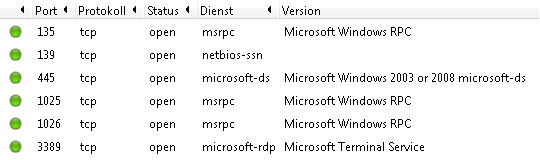
\includegraphics[width=\textwidth,keepaspectratio=true]{Images/dateiserverports}
 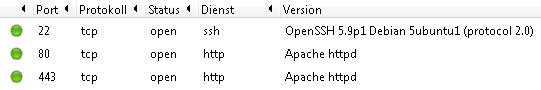
\includegraphics[width=\textwidth,keepaspectratio=true]{Images/webserverports}
 \caption{Offene Ports für Dateiserver (oben) und Webserver (unten)}
 \label{fig:offeneports}
\end{figure}

